\documentclass[11pt]{article}

\usepackage[margin=1in]{geometry}
\usepackage[T1]{fontenc}
\usepackage[utf8]{inputenc}
\usepackage{lmodern}
\usepackage{setspace}
\usepackage{booktabs}
\usepackage{tabularx}
\usepackage{array}
\usepackage{graphicx}
\usepackage{float}
\usepackage{caption}
\usepackage{enumitem}
\usepackage{xcolor}
\usepackage{hyperref}
\usepackage[round,authoryear]{natbib}

\setstretch{1.08}
\setlist[itemize]{leftmargin=1.2em, itemsep=0.2em, topsep=0.4em}
\hypersetup{colorlinks=true, linkcolor=blue!50!black, citecolor=blue!50!black, urlcolor=blue!50!black}

\title{Where Should Economics Test Next?}
\author{Prashant Garg}
\date{\today}

\begin{document}
\maketitle

\begin{abstract}
This note sketches a second paper that asks a different question from the current graph project. The current paper studies missing relations and missing mechanisms. This paper would study missing contexts. The empirical object is a known relation in a setting where it has not yet been studied. Using the current title-and-abstract extraction layer, I show that country context is common enough to support that design, but concentrated enough to make the problem interesting. About 48.5 percent of papers in the concept-edge instance layer carry at least one extracted country context. The corresponding shares are 54.8 percent for concept edges and 69.2 percent for concept nodes. Most tagged papers mention only one country. A much smaller set of nodes and edges span many settings. The note lays out the object, the descriptive margins, and the benchmark designs that could turn context extension into a separate paper on where economics should test next.
\end{abstract}

\section{Introduction}
Economists often care less about whether a relation has ever been studied than about where it has been studied. A paper may establish a relation in the United States, or in China, or in OECD countries, while large parts of the world remain untested. The same issue appears for population groups, firm types, time periods, and institutional settings. If the current graph project asks what relation or mechanism economics should study next, a natural companion question is where economics should test a known relation next.

This note develops that idea as a separate empirical object. The unit is no longer only a relation such as broadband access and business formation, or a mechanism such as broadband access to search frictions to business formation. The unit is a relation paired with a context. A candidate question is therefore not simply whether the literature should study broadband access and business formation. It is whether the literature should study that relation in low-income countries, in rural settings, or after a particular policy shock.

The motivation is substantive, not cosmetic. A large share of economic knowledge is context-bound. That concern sits behind long-standing debates about external validity, heterogeneity, and the transport of evidence across settings \citep{deaton2010instruments,allcott2015site,vivalt2020generalize,hotz2005predicting,bisbee2017local}. Yet most metascience or graph-based discovery objects still focus on missing claims rather than missing coverage of known claims. The present note asks whether the current graph already contains enough context structure to support that second task.

The immediate goal is exploratory. I do not try to estimate a final ranking rule here. I first ask whether the extracted graph contains enough country information, at the paper, edge, and node levels, to make a context-extension paper credible. The answer appears to be yes. The graph already contains a large country-specific substructure. It is broad enough to benchmark. It is also concentrated enough that the problem is not trivial.

\section{Relation to Literature}
This note would sit at the intersection of three literatures.

\subsection{External Validity and Transport Across Settings}
Development and program-evaluation work has long emphasized that credible local estimates do not automatically transport to new settings \citep{deaton2010instruments,allcott2015site,vivalt2020generalize,hotz2005predicting}. That literature usually asks whether an estimated effect generalizes. The graph version of that question asks where the literature appears ready for another test.

\subsection{Scope Conditions and Heterogeneity}
Economists also study when a relation changes with institutions, populations, or macro conditions. In that language, the object here is a coverage gap in scope conditions. The relation is known somewhere, but its support across settings is uneven. That makes the candidate question closer to external validity than to pure relation discovery.

\subsection{Research Allocation}
The current graph paper asks what relation or mechanism the literature should examine next. A context-extension paper would be complementary. It would ask where the literature should take a known relation next. The two papers would therefore share extraction, graph construction, and evaluation ideas, but target different research margins.

\paragraph{Likely contribution.}
The contribution would not be a new estimator of treatment transportability. It would be a prospective ranking problem for context extension. The object is practical: given a known relation, which countries or income groups look most under-studied relative to nearby evidence in the graph?

\section{Data and Empirical Object}
\subsection{Current Context Information in the Graph}
The present graph is already useful for this question because country context is extracted alongside node instances. In the current pipeline, node-level study context is recovered from titles and abstracts. Those extracted contexts are then attached to concept-edge instances. This note therefore uses the same title-and-abstract layer as the main paper, but reads it through a different empirical lens.

The descriptive work below is built from the public concept graph. The key table is the concept-edge instance layer. Each row is an extracted relation from one paper, together with source and target concept IDs, paper title and year, and the country contexts attached to the source and target node instances. I normalize obvious country aliases such as \texttt{USA} and \texttt{United States}, and \texttt{CHN} and \texttt{China}, using the existing context-alias table in the repository.

\subsection{Three Units of Analysis}
There are three useful units for a first pass.

\begin{itemize}
    \item \textbf{Papers.} For each paper, I collect the union of countries that appear anywhere in its extracted node contexts.
    \item \textbf{Concept edges.} For each concept edge, I collect the union of countries across all supporting instances.
    \item \textbf{Concept nodes.} For each concept node, I collect the union of countries across all incident source and target instances.
\end{itemize}

This gives a simple way to ask whether country context is present at all, how concentrated it is, and whether some relations and concepts already span many settings.

\subsection{Candidate Benchmark Object}
The benchmark object for a future paper would be a relation-context pair:
\[
(A \rightarrow B, C),
\]
where the relation \(A \rightarrow B\) already exists in the graph and \(C\) is a country, region, or income-group context in which that relation has not yet been studied. The historical event would be the first later appearance of that relation in context \(C\).

That design is distinct from the current paper's two main objects:
\begin{itemize}
    \item \textbf{Path-to-direct:} a path-supported direct relation later appears.
    \item \textbf{Direct-to-path:} a direct relation later acquires a mechanism path.
\end{itemize}

The proposed context-extension paper would instead ask whether a known relation later travels to a new setting.

\section{Descriptive Evidence}
\subsection{Coverage Across Papers, Edges, and Nodes}
Table \ref{tab:summary} gives the basic coverage facts. The country layer is not universal, but it is substantial. About half of papers and edges carry at least one country context. At the node level, country coverage is more common still.

\begin{table}[H]
\centering
\caption{Country-context coverage across units}
\label{tab:summary}
\begin{tabular}{lrrrrrrr}
\toprule
Unit & N & Share with context & Mean countries & Median & P90 & P99 & Max \\
\midrule
Papers & 27,346 & 48.5\% & 0.6 & 0 & 1 & 5 & 23 \\
Concept edges & 41,738 & 54.8\% & 1.0 & 1 & 2 & 10 & 161 \\
Concept nodes & 6,457 & 69.2\% & 4.3 & 1 & 8 & 49 & 596 \\
\bottomrule
\end{tabular}

\begin{minipage}{0.97\linewidth}
\footnotesize \textit{Notes:} The paper unit is the OpenAlex work ID in the concept-edge instance layer. The edge unit is a concept edge after aggregating over supporting instances. The node unit is a concept node after aggregating over all incident source and target instances. Country context is recovered from extracted title-and-abstract study-context fields. Alias normalization collapses obvious duplicates such as \texttt{USA} and \texttt{United States}. The table reports the share of units with any country context, together with the distribution of the number of unique normalized countries linked to each unit.
\end{minipage}
\end{table}

Figure \ref{fig:coverage} shows the distribution more directly. Most tagged papers mention a single country. By contrast, country breadth expands quickly at the edge and node levels because repeated instances accumulate across papers and settings. This is the descriptive fact that makes the idea viable. The literature is neither context-free nor evenly covered.

\begin{figure}[H]
\centering
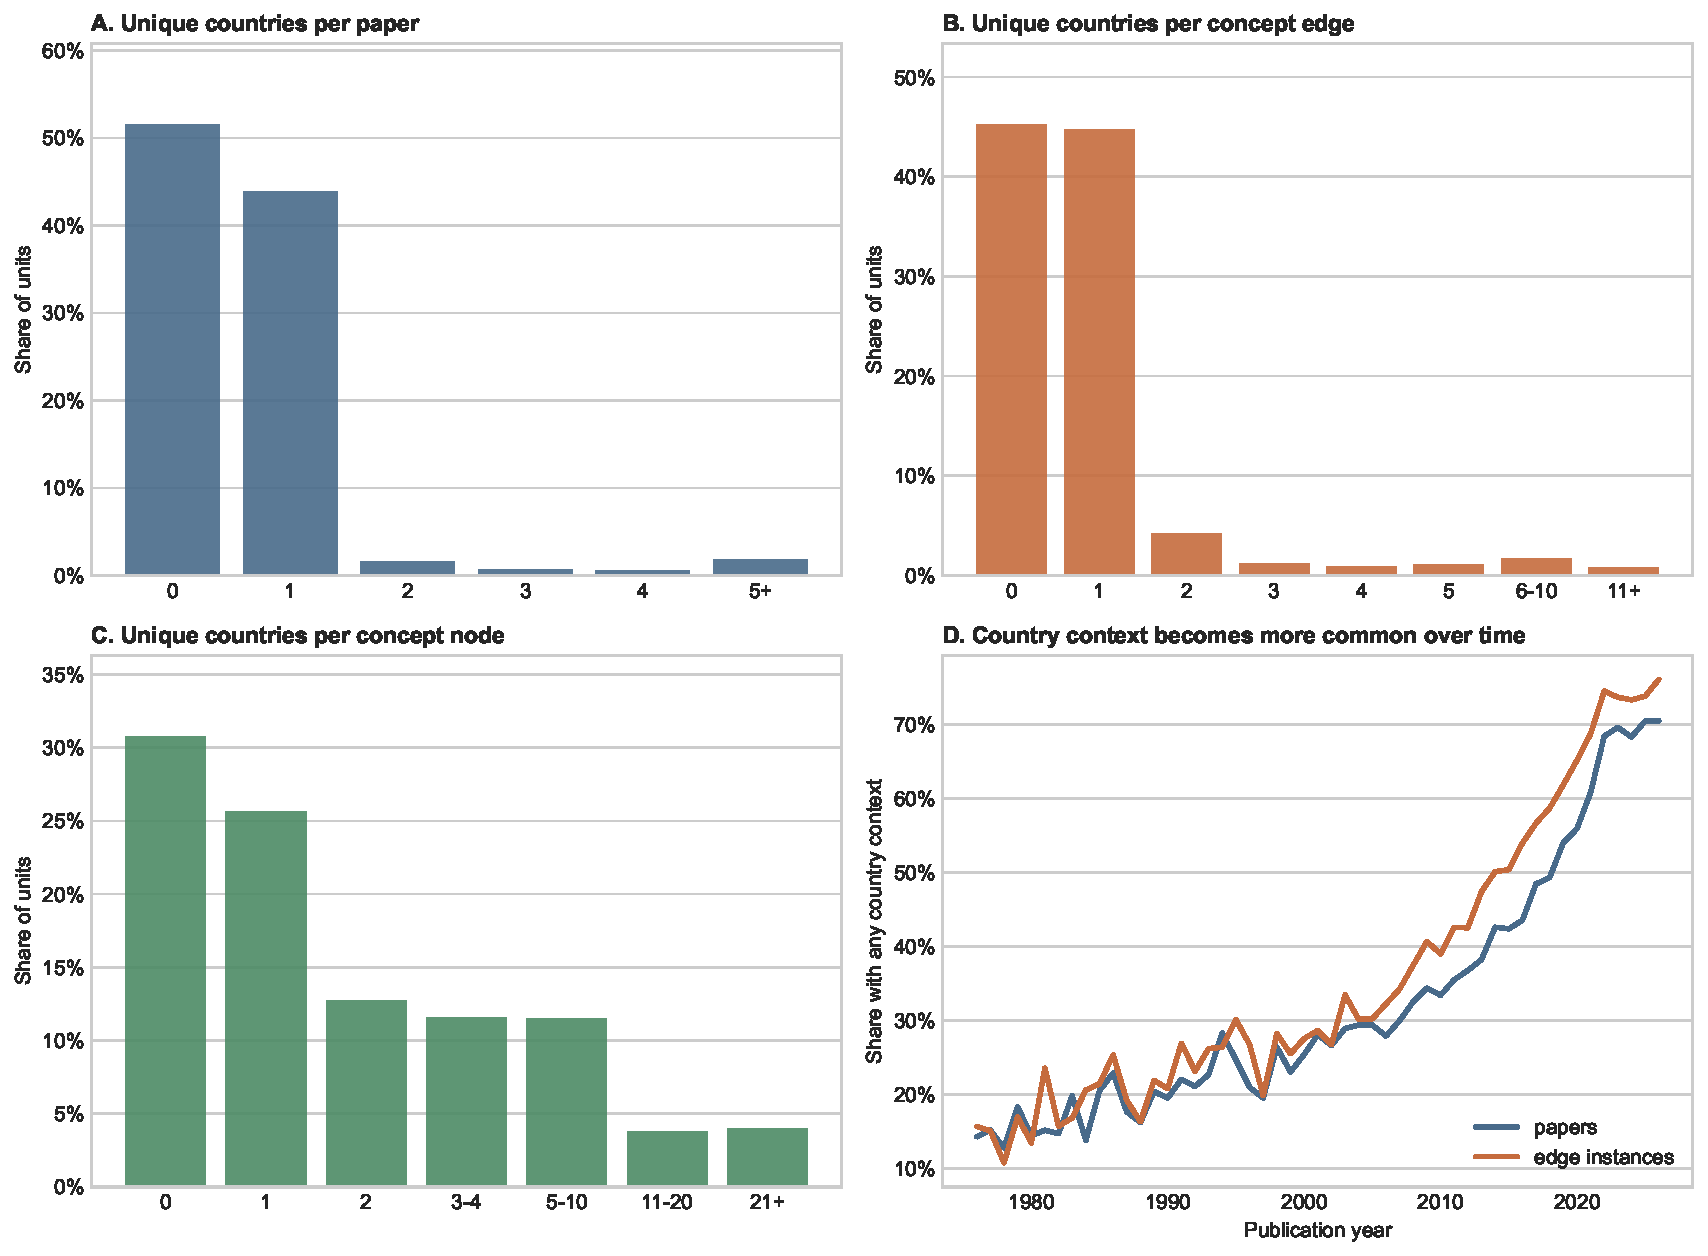
\includegraphics[width=\linewidth]{figures/context_coverage_distributions.pdf}
\caption{Country-context coverage across papers, edges, and nodes}
\label{fig:coverage}
\begin{minipage}{0.97\linewidth}
\footnotesize \textit{Notes:} Panel A shows the distribution of the number of unique normalized countries linked to each paper through extracted node contexts. Panel B shows the same object for concept edges after aggregating across supporting instances. Panel C shows the same object for concept nodes after aggregating across all incident instances. Panel D reports the yearly share of papers and edge instances with any country context. All country counts use the existing context-alias normalization table.
\end{minipage}
\end{figure}

\subsection{Concentration Across Countries}
Country context is also highly concentrated. China and the United States dominate across all three units. A separate tier of countries appears often enough to support a context-extension exercise, but the long tail remains thin. That is exactly the pattern one would want if the paper is about where economics should test next. A fully even distribution would leave little to rank. A nearly empty distribution would leave nothing to rank.

\begin{figure}[H]
\centering
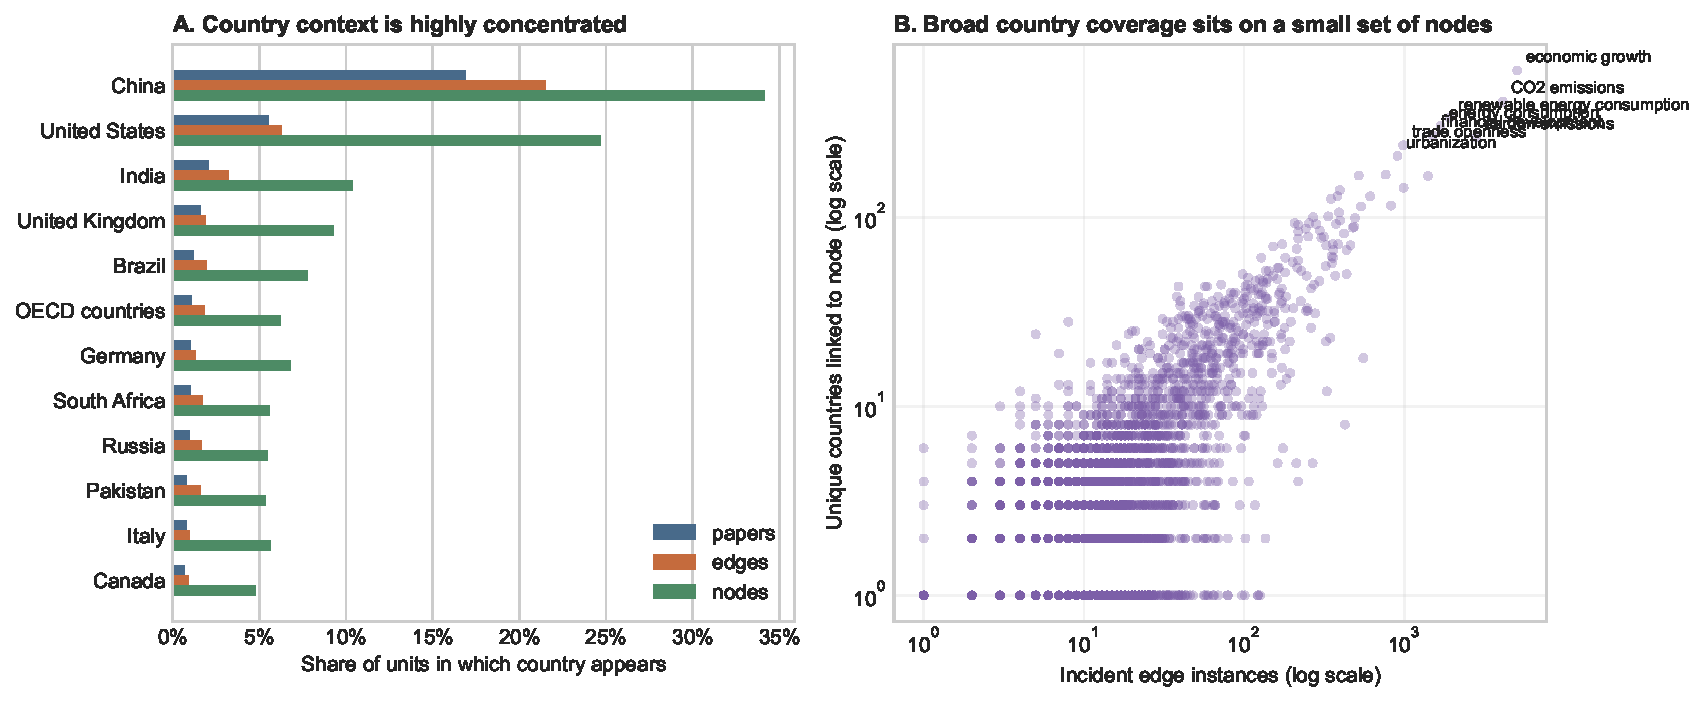
\includegraphics[width=\linewidth]{figures/context_concentration_and_scope.pdf}
\caption{Country concentration and cross-setting breadth}
\label{fig:concentration}
\begin{minipage}{0.97\linewidth}
\footnotesize \textit{Notes:} Panel A shows the share of papers, concept edges, and concept nodes in which each of the top twelve countries appears at least once. Panel B plots, for each concept node with at least one country context, the number of incident edge instances against the number of unique normalized countries linked to that node. Both axes in Panel B use log scales. Labels mark the nodes with the broadest country footprint.
\end{minipage}
\end{figure}

\subsection{Which Relations Already Span Many Settings?}
Table \ref{tab:topnodes} and Table \ref{tab:topedges} list the nodes and edges with the widest country spread. The results are instructive. The broadest nodes are macro and environment concepts such as economic growth, CO\textsubscript{2} emissions, renewable energy consumption, and trade openness. The broadest edges are similarly familiar: growth and emissions, energy use and emissions, and other high-volume macro-development relations. This suggests that a first context-extension paper will likely begin with broad literatures. A second step would be to ask whether narrower relations also show enough context structure once one moves beyond country to income group or region.

\begin{table}[H]
\centering
\caption{Concept nodes with the widest country footprint}
\label{tab:topnodes}
\begin{tabular}{p{7.5cm}rr}
\toprule
Node & Unique countries & Incident instances \\
\midrule
economic growth & 596 & 5,070 \\
CO2 emissions & 408 & 4,119 \\
renewable energy consumption & 335 & 1,925 \\
energy consumption & 303 & 1,683 \\
financial development & 271 & 1,507 \\
carbon emissions & 264 & 2,806 \\
trade openness & 240 & 985 \\
urbanization & 211 & 907 \\
foreign direct investments & 168 & 765 \\
renewable energy & 166 & 520 \\
\bottomrule
\end{tabular}

\begin{minipage}{0.97\linewidth}
\footnotesize \textit{Notes:} The table ranks concept nodes by the number of unique normalized countries linked to that node across all incident source and target instances. Incident instances count the number of concept-edge instances in which the node appears.
\end{minipage}
\end{table}

\begin{table}[H]
\centering
\caption{Concept edges with the widest country footprint}
\label{tab:topedges}
\begin{tabular}{p{8.5cm}rr}
\toprule
Edge & Unique countries & Supporting instances \\
\midrule
economic growth -> CO2 emissions & 161 & 330 \\
economic growth -> carbon emissions & 101 & 202 \\
energy consumption -> economic growth & 101 & 173 \\
renewable energy consumption -> economic growth & 99 & 183 \\
economic growth -> renewable energy consumption & 94 & 104 \\
renewable energy consumption -> CO2 emissions & 89 & 161 \\
economic growth -> energy consumption & 85 & 133 \\
energy consumption -> CO2 emissions & 84 & 158 \\
financial development -> CO2 emissions & 74 & 128 \\
economic growth -> ecological footprint & 73 & 123 \\
\bottomrule
\end{tabular}

\begin{minipage}{0.97\linewidth}
\footnotesize \textit{Notes:} The table ranks concept edges by the number of unique normalized countries linked to the edge across all supporting instances. Supporting instances count the number of concept-edge instances attached to the edge.
\end{minipage}
\end{table}

\subsection{What the Descriptives Already Suggest}
These descriptives point to four preliminary conclusions.

\begin{itemize}
    \item The graph already contains enough explicit country structure to support a context-extension paper.
    \item The distribution is skewed enough that ranking is meaningful. Some relations are already global. Many remain narrow.
    \item Broad country coverage is concentrated in high-volume nodes and edges. That suggests the first benchmark will likely live in literatures with large repeated support.
    \item Country context becomes more common over time. That helps the prospective design because later years offer a thicker context margin than the earliest part of the sample.
\end{itemize}

\section{Candidate Research Designs}
\subsection{Relation-Context Extension}
The cleanest first object is a known relation in a new setting. Suppose the graph already contains broadband access and business formation in several countries, but not in lower-income settings or rural economies. A context-extension candidate asks whether the relation should be tested there next.

\paragraph{Historical event.}
Freeze the graph at year \(t-1\). Observe that relation \(A \rightarrow B\) exists, but not in context \(C\). Rank candidate triples \((A \rightarrow B, C)\). Check whether the literature later studies that relation in \(C\).

\paragraph{Likely baseline comparisons.}
\begin{itemize}
    \item context popularity alone
    \item relation popularity alone
    \item simple combinations of relation support and context frequency
    \item graph-informed transfer from nearby contexts
\end{itemize}

\paragraph{Likely graph features.}
\begin{itemize}
    \item how often the relation appears in nearby countries
    \item how often adjacent relations appear in the target context
    \item whether the target context is under-covered relative to the size of the surrounding literature
    \item whether the relation already appears in related income groups or regions
\end{itemize}

\subsection{Mechanism-Context Extension}
The second object is a known mechanism in a new setting. Suppose the literature already studies transit investment, commuting time, and employment in several countries. The context question becomes whether the same mechanism should be tested in a new setting. This is closer to the direct-to-path object in the current paper, but now the missing margin is context rather than mechanism itself.

\subsection{Country to Income-Group Extension}
Country is the right starting point because it is explicit and relatively easy to extract. But country alone may be too granular. A practical next version would map countries to broader categories:
\begin{itemize}
    \item World Bank income groups
    \item region
    \item advanced versus emerging or developing economies
    \item state capacity or institutional-quality bins
\end{itemize}
This would reduce sparsity and move the paper closer to questions economists often ask in practice.

\subsection{Time-Period Extension}
Another branch is temporal rather than geographic. A relation may be well studied in pre-2008 data and thin in later macro conditions. The unit would then be a relation-time-period pair rather than a relation-country pair. I do not build that design here, but it belongs in the same family.

\section{What Could Stay in the Current Paper, and What Likely Becomes Separate}
Some parts of this idea could support the current paper. A small appendix or discussion section could note that known relations are also unevenly distributed across countries, and that context extension is a natural next object once relation and mechanism discovery are established.

The full empirical design likely deserves its own paper. The reason is not only length. The benchmark object changes. The ranking targets change. The baseline comparisons change. The interpretation also changes. The current paper asks what economics should study next. This paper would ask where economics should test a known relation next.

\paragraph{How the two papers would fit together.}
\begin{itemize}
    \item \textbf{Current paper:} missing relation or missing mechanism
    \item \textbf{Next paper:} missing setting for a known relation
\end{itemize}

\section{Open Empirical Tasks}
The descriptives above are enough to justify a serious next step, but several design choices remain open.

\subsection{Immediate Tasks}
\begin{itemize}
    \item Build a clean relation-context panel for historical validation.
    \item Compare country, region, and income-group contexts.
    \item Decide whether the benchmark should require a direct relation to exist before a new context can be proposed.
    \item Decide whether a context-extension object should be paired with path-to-direct and direct-to-path in the same broad program of work, or written as a separate paper.
\end{itemize}

\subsection{Additional Descriptives Worth Adding}
\begin{itemize}
    \item distribution of context coverage by field bucket
    \item distribution of context coverage by publication year and journal tier
    \item concentration curves for countries and income groups
    \item country breadth conditional on node support
    \item edge breadth conditional on whether the edge is causal, correlational, or mechanism-heavy
    \item country-pair or region-pair descriptives for relations that travel together across settings
    \item the same descriptive panels for time periods and income groups, once those tags are materialized cleanly
\end{itemize}

\subsection{Longer-Run Extensions}
There is also a more open-ended third object: not only missing contexts for known relations, but settings or populations that are missing from the graph more generally. That is conceptually interesting, but it should come after relation-context benchmarking rather than before it.

\section{Conclusion}
The present graph already contains enough country structure to support a context-extension agenda. The simplest version is clear: take a known relation, ask where it has not yet been studied, and rank those missing settings prospectively. The descriptive evidence suggests that this is neither empty nor trivial. A substantial share of the graph already carries explicit country context. At the same time, that context is highly concentrated across countries, nodes, and edges. That is exactly the pattern that makes a ranking problem worth studying.

This note therefore supports a concrete next step. Finish the current two-object paper. Then build a second paper around relation-context extension, starting with countries and likely moving next to income groups and time periods.

\bibliographystyle{apalike}
\bibliography{context_extension_paper}

\end{document}
